% =========================================
% system_analysis_requirements.tex
% =========================================

\chapter{System Analysis and Requirements}\label{chapter:analysis}

% -----------------------------------------
% 3.1 INTRODUCTION (mapped to sec:analysis:reqs)
% -----------------------------------------
\section{Introduction}\label{sec:analysis:reqs}
This chapter presents a detailed analysis of the MedEcho medical AI system from a requirements and stakeholder perspective. It identifies who interacts with the system, what the system must accomplish, and the constraints under which it must operate. The goal of this chapter is to define the functional and non-functional requirements that guide the system design and ensure that MedEcho can be safely and effectively deployed in a real clinical environment.



% -----------------------------------------
% 3.2 STAKEHOLDER ANALYSIS
% -----------------------------------------
\section{Stakeholder Analysis}
\label{sec:analysis:analysis} 
MedEcho is used within a complex healthcare ecosystem involving multiple stakeholders. Each stakeholder group has different goals, responsibilities, and expectations from the system. Understanding these stakeholders is essential to ensure that the system satisfies clinical, technical, and administrative needs.

Doctors are the primary users who interact with the system during patient consultations. Hospital administrators and IT staff are responsible for deployment, maintenance, and compliance. Patients are indirect stakeholders whose data must be protected. University supervisors are also stakeholders, as MedEcho is used for OSCE-based academic evaluation and training.

Additionally, AI Developers and Researchers are stakeholders who monitor the system’s performance metrics, such as transcription accuracy and the effectiveness of the Local Knowledge Layer (LKL) in mitigating hallucinations.


% -----------------------------------------
% 3.3 FUNCTIONAL REQUIREMENTS
% -----------------------------------------
\section{Functional Requirements}\label{sec:analysis:functional}

The core functional requirements of MedEcho are as follows:

\begin{itemize}
    \item \textbf{Audio Capture \& Pre-processing:} Record patient intake audio with noise-handling capabilities to ensure high-quality input for the AI model.

    \item \textbf{AI-Driven Transcription:} Utilize OpenAI Whisper to perform robust speech-to-text transcription of clinical dictations.

    \item \textbf{Intelligent Report Structuring (Phase~1):} Apply prompt engineering with large language models to transform transcribed text into an OSCE-compliant structured JSON report for patient intake.

    \item \textbf{Local Data Management:} Store case data locally (e.g., in \texttt{memory.json}) to ensure privacy, security, and offline availability.

    \item \textbf{Multi-Phase Assessment Recording:} Capture the final clinical assessment separately (Phase~2) to maintain a logical and clinically aligned workflow.

    \item \textbf{Intelligent Report Merging:} Automatically integrate and synchronize Phase~1 and Phase~2 outputs into a unified, consistent medical record.

    \item \textbf{Local Knowledge Layer (LKL) Update:} Dynamically update the system’s knowledge using new cases to adapt to hospital-specific terminology and reduce hallucinations.

    \item \textbf{Human-in-the-Loop Verification:} Allow physicians to review, edit, and validate AI-generated reports before finalization to ensure clinical correctness.

    \item \textbf{Professional Documentation Export:} Generate final reports in PDF format for archiving and provide JSON exports for interoperability with other systems.
\end{itemize}

These functional requirements define the complete clinical documentation workflow supported by MedEcho. The system is designed around a two-phase process in which patient intake information and final clinical assessment are captured separately and later merged into a single, consistent medical record. This approach ensures both completeness and traceability of clinical data.





% -----------------------------------------
% 3.4 NON-FUNCTIONAL REQUIREMENTS
% -----------------------------------------
\section{Non-Functional Requirements}\label{sec:analysis:nfr}

Non-functional requirements are critical in healthcare environments, where system reliability, data protection, and usability directly affect patient safety and clinician efficiency. The following requirements define the expected quality attributes of MedEcho, with a particular focus on AI inference performance, privacy, and deployability.

% -----------------------------------------
% 3.4.1 PERFORMANCE & AI INFERENCE REQUIREMENTS
% -----------------------------------------
\subsection{Performance \& AI Inference Requirements}\label{sec:analysis:nfr:performance}

\begin{itemize}
    \item \textbf{Inference Latency (Speech-to-Text):} The Whisper-based ASR pipeline must achieve near real-time inference such that transcription latency does not significantly exceed the duration of the input audio on the target hospital hardware, enabling interactive clinical use during live consultations.

    \item \textbf{LLM Response Latency:} The LLM-based report structuring and merging stages must be optimized to generate OSCE-compliant structured outputs within clinically acceptable response times, ensuring a smooth end-user experience.

    \item \textbf{Resource Efficiency:} The AI pipeline shall manage CPU/GPU utilization and memory consumption effectively (e.g., memory-efficient model loading and controlled batching) to maintain system stability during heavy inference workloads.

    \item \textbf{Pipeline Efficiency:} The system should minimize end-to-end latency by reducing idle time between stages (audio processing, transcription, structuring, validation, and report generation) while preserving output quality and correctness.

    \item \textbf{Performance Under Load:} The system must maintain predictable response times when processing multiple sessions or requests, supporting peak outpatient usage without severe degradation.
\end{itemize}

% -----------------------------------------
% 3.4.2 SECURITY & DATA PRIVACY REQUIREMENTS
% -----------------------------------------
\subsection{Security \& Data Privacy Requirements}\label{sec:analysis:nfr:security}

\begin{itemize}
    \item \textbf{Local Inference \& Privacy:} To comply with healthcare data protection standards, clinical audio, transcripts, and report generation must be performed locally whenever possible, minimizing exposure of sensitive patient data to external services.

    \item \textbf{Role-Based Access Control (RBAC):} The system shall enforce strict access levels for different user categories (e.g., Doctor, Administrator, IT Staff), ensuring data integrity and preventing unauthorized operations.

    \item \textbf{Data Encryption:} All locally stored medical records (JSON/PDF), configuration files, and system logs containing clinical identifiers must be protected using industry-standard encryption mechanisms.

    \item \textbf{Auditability:} The system should maintain basic audit logs for critical actions (e.g., report generation, export, deletion/archiving, user login) to support accountability and troubleshooting.
\end{itemize}

% -----------------------------------------
% 3.4.3 USABILITY & HUMAN-CENTRIC DESIGN
% -----------------------------------------
\subsection{Usability \& Human-Centric Design}\label{sec:analysis:nfr:usability}

\begin{itemize}
    \item \textbf{Professional UI/UX:} A streamlined, medical-themed interface (Electron-based) shall be provided to minimize cognitive load and allow clinicians to complete documentation with minimal friction.

    \item \textbf{Intuitive Workflow:} The user flow must require a minimal number of steps for recording, previewing, editing, and finalizing reports, with clear feedback for system states (recording, processing, completed, error).

    \item \textbf{Human-in-the-Loop Validation:} The system shall allow physicians to review, edit, and validate AI-generated content before finalization, supporting clinical correctness and accountability.

    \item \textbf{Bilingual Support:} The system should support Arabic and English text processing and display to match local clinical needs and improve usability.
\end{itemize}

% -----------------------------------------
% 3.4.4 SCALABILITY & MODULAR ARCHITECTURE
% -----------------------------------------
\subsection{Scalability \& Modular Architecture}\label{sec:analysis:nfr:scalability}

\begin{itemize}
    \item \textbf{Deployment Scalability:} The architecture must support deployment across multiple clinics or hospital departments without requiring major redesign, enabling gradual rollout and expansion.

    \item \textbf{Modular Backend:} The backend shall follow a modular design where key components (Whisper, LLM services, PDF generator, and the Local Knowledge Layer) can be updated, replaced, or scaled independently without impacting overall system stability.

    \item \textbf{Maintainability:} The system should support clear separation of concerns and well-defined interfaces between modules to simplify debugging, testing, and future upgrades.

    \item \textbf{Interoperability:} The system should support exporting structured data (JSON) to facilitate integration with other clinical systems when required.
\end{itemize}


% -----------------------------------------
% 3.5 SYSTEM MODELING
% -----------------------------------------
\section{System Modeling}\label{sec:analysis:modeling}

This section presents abstract models that describe how users interact with MedEcho and how the system behaves during a typical clinical session. The models focus on the functional behavior of the system rather than implementation details.
\subsection{Use Case Diagram}\label{sec:analysis:usecases}

The use case model summarizes the main interactions between users and the MedEcho system. The primary actor is the physician, who performs actions related to clinical documentation, while secondary actors include hospital administrators and IT staff.

The main use cases supported by MedEcho include:



\begin{itemize}
    \item Record intake audio.
    \item Transcribe audio.
    \item Generate structured report.
    \item Merge Phase~1 and Phase~2 reports.
    \item Save and load cases.
    \item Export PDF.
    \item Update the Local Knowledge Layer (LKL).
\end{itemize}
The use case diagram in Figure~\ref{fig:Use case diagram} shows that MedEcho is centered around two main clinical phases: patient intake and final assessment. These two phases ensure that all relevant clinical information is captured, structured, and stored in a consistent manner.

\begin{figure}[H]
\centering
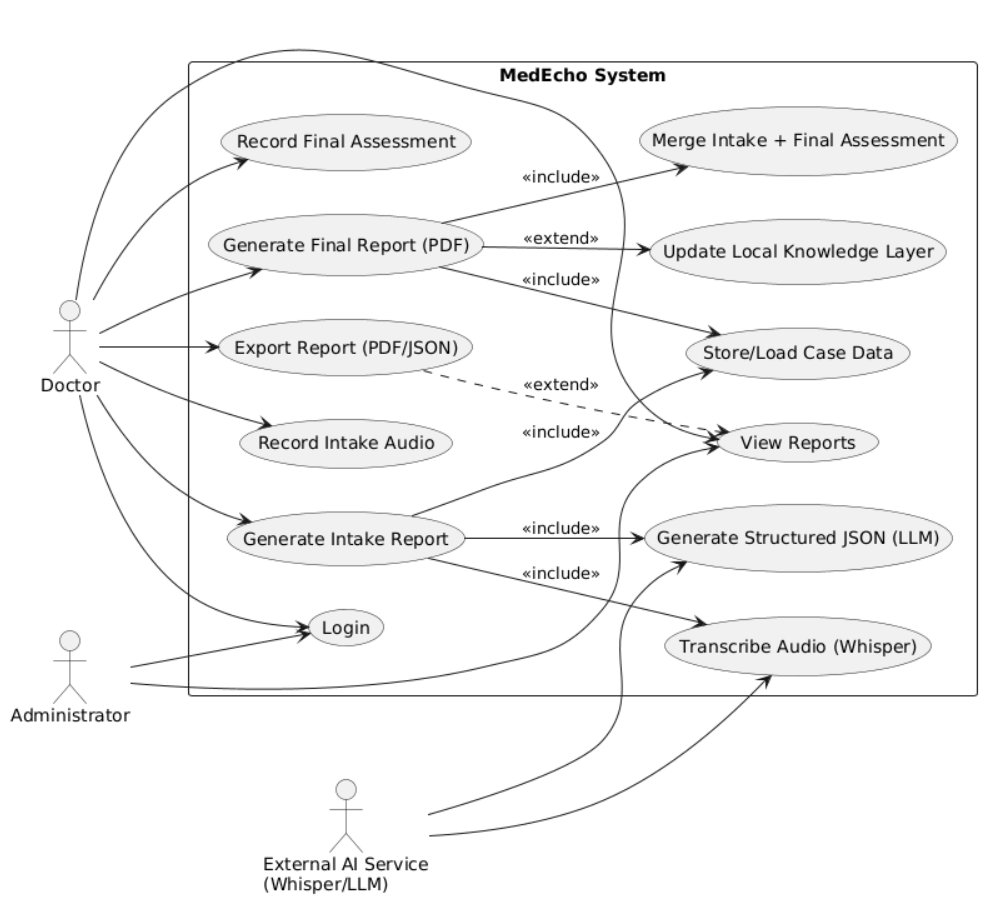
\includegraphics[width=\textwidth]{img/use case .png}
\caption{Use case diagram for MedEcho .}
\label{fig:Use case diagram}
\end{figure}

\subsection{Activity Diagram — Phase 1}\label{sec:analysis:activity1}

Phase~1 represents the patient intake workflow. During this phase, the physician records the patient’s medical history and symptoms, which are automatically processed by MedEcho to create an initial structured clinical record.

\begin{enumerate}
    \item The doctor starts recording intake audio.
    \item Whisper generates a text transcript from the audio.
    \item GPT converts the transcript into an OSCE-based JSON structure.
    \item The JSON record is saved locally.
    \item A preview of the structured report is shown in the UI.
\end{enumerate}

\begin{figure}[ht]
    \centering
    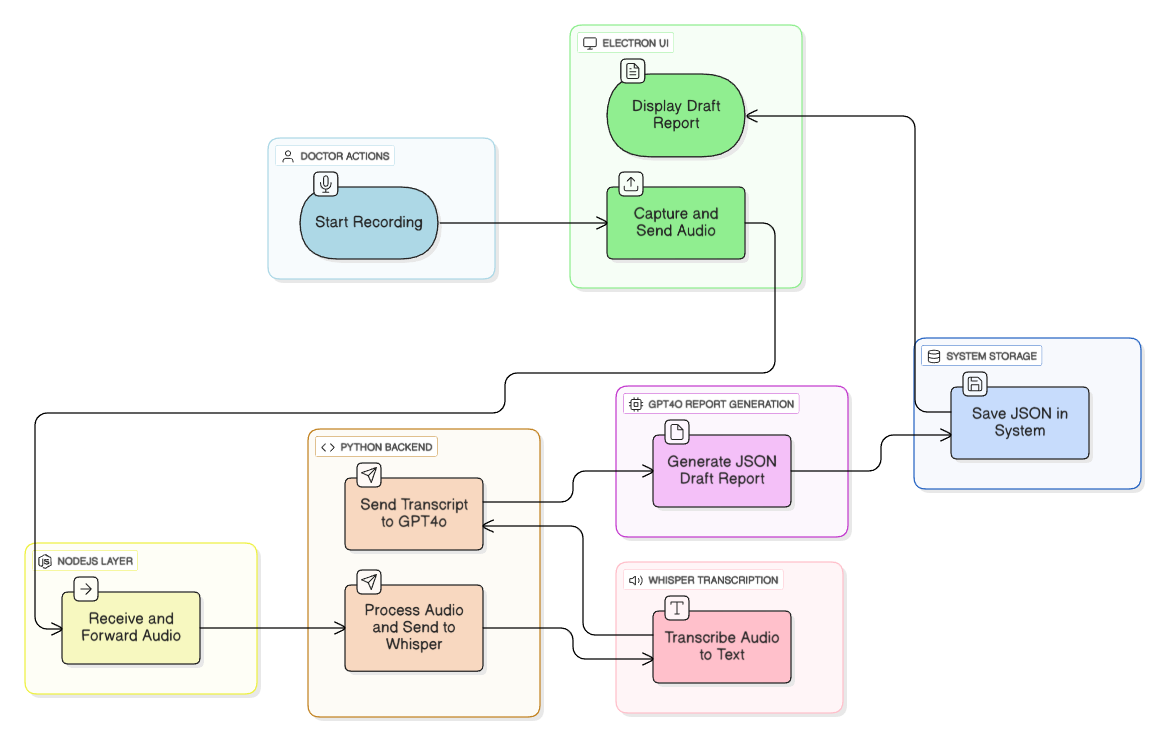
\includegraphics[width=\textwidth]{img/phase 1 activity.png}
    \caption{Phase 1 activity diagram .}
    \label{fig:activity1}
\end{figure}
This activity diagram illustrates how MedEcho transforms spoken clinical input into a structured OSCE-compliant record. By automating transcription and structuring, the system reduces manual data entry while maintaining consistency and completeness.

\subsection{Activity Diagram — Phase 2}\label{sec:analysis:activity2}

Phase~2 corresponds to the final clinical assessment. In this phase, the physician records diagnostic conclusions and clinical decisions, which are merged with the previously captured intake data to form a complete medical report.


\begin{enumerate}
    \item The doctor records the final clinical dictation.
    \item Whisper produces the final text.
    \item GPT merges the final dictation with the Phase~1 JSON record.
    \item A final PDF report is generated.
    \item The complete case is stored in local history.
\end{enumerate}
This phase ensures that preliminary and final clinical information are integrated into a single coherent record, which is then stored and exported as a professionally formatted medical report.




% -----------------------------------------
% 3.6 SYSTEM SEQUENCE DIAGRAMS
% -----------------------------------------
\section{System Sequence Diagrams}\label{sec:analysis:seq}

Sequence diagrams are used to describe how different components of MedEcho interact during a typical clinical session. These sequences illustrate the flow of control and data between the user interface, backend services, and AI components.


\subsection*{Phase 1 Sequence}

During Phase~1, MedEcho captures patient intake information and transforms it into a structured clinical record. The interaction sequence ensures that audio, text, and structured data flow through the system in a controlled and traceable manner.

\begin{enumerate}
    \item Doctor interacts with the Electron UI.
    \item Electron UI sends requests to the Node.js backend.
    \item Node.js forwards audio and metadata to the Python backend.
    \item Python services call Whisper for transcription.
    \item Transcribed text is passed to GPT for structuring.
    \item Structured data is returned to the UI and stored locally.
\end{enumerate}


\subsection*{Phase 2 Sequence}



Phase~2 focuses on generating the final clinical report. In this phase, new spoken input is combined with the previously captured intake data to produce a complete and professionally formatted medical document.


\begin{enumerate}
    \item Doctor records final dictation via the UI.
    \item Backend sends audio to Whisper for transcription.
    \item GPT merges the new text with Phase~1 JSON.
    \item PDF generator creates the final report.
    \item The UI displays the final PDF and saves the case.
\end{enumerate}




% -----------------------------------------
% 3.7 DATA FLOW DIAGRAMS (DFD)
% -----------------------------------------
\section{Data Flow Diagrams (DFD)}\label{sec:analysis:dfd}

Data flow diagrams describe how information moves through MedEcho from the moment it is recorded until it becomes a finalized medical report. These diagrams emphasize the separation between data acquisition, processing, and storage.

\subsection*{DFD Level 0}



At Level~0, MedEcho is viewed as a single system that transforms spoken clinical input into structured and persistent medical documentation.

\begin{itemize}
    \item receives audio input from the doctor,
    \item uses Whisper to obtain text,
    \item uses GPT to generate structured JSON,
    \item passes JSON to the PDF generator to produce a report.
\end{itemize}

\subsection*{DFD Level 1}

Level~1 expands the internal processes of MedEcho and shows how audio, text, and structured data are processed and validated before being stored and exported.

\begin{itemize}
    \item preprocessing of audio,
    \item segmentation and batching for Whisper,
    \item prompt construction for GPT,
    \item validation and post-processing of JSON fields,
    \item PDF layout generation and file storage.
\end{itemize}



% -----------------------------------------
% 3.8 REQUIREMENTS TABLE (mapped to sec:analysis:stories)
% -----------------------------------------
\section{Requirements Table}\label{sec:analysis:stories}
Table~\ref{tab:reqs} illustrates a sample of functional and non-functional requirements.
The selection of tools and technologies was guided by the need for reliability, modularity, and compliance with medical data processing requirements.
s


\begin{table}[ht]
\centering
\renewcommand{\arraystretch}{1.3}
\setlength{\tabcolsep}{6pt}
\begin{tabular}{|c|c|p{7cm}|c|}
\hline
\textbf{ID} & \textbf{Type} & \textbf{Description} & \textbf{Priority} \\
\hline
FR-01 & Functional       & Record intake audio from the doctor. & High \\
\hline
FR-02 & Functional       & Transcribe audio using Whisper. & High \\
\hline
FR-07 & Functional       & Generate final PDF report from structured data. & High \\
\hline
NFR-02 & Non-Functional & Provide offline capability on local servers. & High \\
\hline
NFR-04 & Security       & Support role-based access for different user roles. & High \\
\hline
\end{tabular}
\caption{Sample of MedEcho requirements in structured tabular form.}
\label{tab:reqs}
\end{table}
This table ensures traceability between high-level system objectives and concrete implementation requirements. It also allows verification that all critical clinical and security needs are addressed by the system.


% -----------------------------------------
% 3.9 TOOLS AND TECHNOLOGIES
% -----------------------------------------
\section{Tools and Technologies}\label{sec:analysis:tools}

The selection of tools and technologies was guided by the need for reliability, modularity, and compliance with medical data processing requirements.


\begin{table}[ht]
\centering
\renewcommand{\arraystretch}{1.3}
\begin{tabular}{|p{4cm}|p{9cm}|}
\hline
\textbf{Layer} & \textbf{Technology} \\
\hline
User Interface (UI) & Electron with HTML/CSS and TailwindCSS components. \\
\hline
Backend Services & Node.js for application logic and API routing. \\
\hline
AI Layer & Python services using Whisper and GPT-based models. \\
\hline
Storage & Local JSON files and structured report archives. \\
\hline
Knowledge Layer & LKL (Local Knowledge Layer) that learns from hospital cases. \\
\hline
\end{tabular}
\caption{Tools and technologies used in MedEcho.}
\label{tab:tech-stack}
\end{table}
This layered technology stack allows MedEcho to separate user interaction, AI processing, and data management, enabling easier maintenance, scalability, and future upgrades.


% -----------------------------------------
% 3.10 REGULATORY AND ETHICAL CONSIDERATIONS
% -----------------------------------------
\section{Regulatory and Ethical Considerations}\label{sec:analysis:ethics}

MedEcho is designed with privacy and ethical considerations in mind:

\begin{itemize}
    \item No patient data is stored or processed on external cloud services without explicit approval.
    \item All primary processing is performed locally on hospital-controlled infrastructure.
    \item The system follows medical privacy principles similar to HIPAA-style guidelines.
    \item A ``no hallucinations'' policy is enforced: generated content is constrained by clinical templates and LKL knowledge.
    \item The Local Knowledge Layer improves accuracy while respecting data governance policies.
\end{itemize}
These measures ensure that MedEcho operates as a clinical support tool rather than a decision-making system, preserving physician responsibility while improving documentation quality and efficiency.
